\documentclass[]{article}
\usepackage{lmodern}
\usepackage{amssymb,amsmath}
\usepackage{ifxetex,ifluatex}
\usepackage{fixltx2e} % provides \textsubscript
\ifnum 0\ifxetex 1\fi\ifluatex 1\fi=0 % if pdftex
  \usepackage[T1]{fontenc}
  \usepackage[utf8]{inputenc}
\else % if luatex or xelatex
  \ifxetex
    \usepackage{mathspec}
  \else
    \usepackage{fontspec}
  \fi
  \defaultfontfeatures{Ligatures=TeX,Scale=MatchLowercase}
\fi
% use upquote if available, for straight quotes in verbatim environments
\IfFileExists{upquote.sty}{\usepackage{upquote}}{}
% use microtype if available
\IfFileExists{microtype.sty}{%
\usepackage{microtype}
\UseMicrotypeSet[protrusion]{basicmath} % disable protrusion for tt fonts
}{}
\usepackage[margin=1in]{geometry}
\usepackage{hyperref}
\hypersetup{unicode=true,
            pdftitle={Merge},
            pdfauthor={Ciellie Jansen van Vuuren},
            pdfborder={0 0 0},
            breaklinks=true}
\urlstyle{same}  % don't use monospace font for urls
\usepackage{longtable,booktabs}
\usepackage{graphicx,grffile}
\makeatletter
\def\maxwidth{\ifdim\Gin@nat@width>\linewidth\linewidth\else\Gin@nat@width\fi}
\def\maxheight{\ifdim\Gin@nat@height>\textheight\textheight\else\Gin@nat@height\fi}
\makeatother
% Scale images if necessary, so that they will not overflow the page
% margins by default, and it is still possible to overwrite the defaults
% using explicit options in \includegraphics[width, height, ...]{}
\setkeys{Gin}{width=\maxwidth,height=\maxheight,keepaspectratio}
\IfFileExists{parskip.sty}{%
\usepackage{parskip}
}{% else
\setlength{\parindent}{0pt}
\setlength{\parskip}{6pt plus 2pt minus 1pt}
}
\setlength{\emergencystretch}{3em}  % prevent overfull lines
\providecommand{\tightlist}{%
  \setlength{\itemsep}{0pt}\setlength{\parskip}{0pt}}
\setcounter{secnumdepth}{5}
% Redefines (sub)paragraphs to behave more like sections
\ifx\paragraph\undefined\else
\let\oldparagraph\paragraph
\renewcommand{\paragraph}[1]{\oldparagraph{#1}\mbox{}}
\fi
\ifx\subparagraph\undefined\else
\let\oldsubparagraph\subparagraph
\renewcommand{\subparagraph}[1]{\oldsubparagraph{#1}\mbox{}}
\fi

%%% Use protect on footnotes to avoid problems with footnotes in titles
\let\rmarkdownfootnote\footnote%
\def\footnote{\protect\rmarkdownfootnote}

%%% Change title format to be more compact
\usepackage{titling}

% Create subtitle command for use in maketitle
\newcommand{\subtitle}[1]{
  \posttitle{
    \begin{center}\large#1\end{center}
    }
}

\setlength{\droptitle}{-2em}
  \title{Merge}
  \pretitle{\vspace{\droptitle}\centering\huge}
  \posttitle{\par}
  \author{Ciellie Jansen van Vuuren}
  \preauthor{\centering\large\emph}
  \postauthor{\par}
  \predate{\centering\large\emph}
  \postdate{\par}
  \date{3/2/2018}

\usepackage{booktabs}
\usepackage{longtable}
\usepackage{array}
\usepackage{multirow}
\usepackage[table]{xcolor}
\usepackage{wrapfig}
\usepackage{float}
\usepackage{colortbl}
\usepackage{pdflscape}
\usepackage{tabu}
\usepackage{threeparttable}

\usepackage{ragged2e}
\usepackage{placeins}

\begin{document}
\maketitle

\begin{center}\rule{0.5\linewidth}{\linethickness}\end{center}

\hypertarget{introduction}{%
\section{Introduction}\label{introduction}}

Grubbs catalysts for alkene metathesis have a vast range of advantages,
but the fact that these catalysts are homogeneous makes extraction of
the catalyst from the post-reaction mixtures very difficult. Because of
cost implications, the re-use of the catalyst became very important
(Jordaan, 2007).

A heterogeneous catalyst can be a solution to the above-mentioned issue.
In general, the activity and selectivity of heterogeneous catalysts are
lower than homogeneous catalysts, but the advantage of separation,
recovery and recycling outweigh these shortcomings.

According to literature mesoporous support materials, are ideal
heterogeneous support materials (Thielemann \emph{et al.}, 2011),(Balcar
\& Čejka, 2013). In this study, we decided to focus on the SBA-15 and
MCM-41 mesoporous support material.

The first step in modelling a SBA-15 or MCM-41 mesoporous surface is to
create an amorphous SiO2 bulk using an alpha-quartz (space group 180).
(Balcar \& Čejka, 2013) The 3X3X3 super cell was submitted to dynamics
studies using Materials Studio's CASTEP module and VASP 5.3 (Izumi
\emph{et al.}, 2004),(Ugliengo \emph{et al.}, 2008). This was done and I
will discuss the procedure that I followed to accomplish this.

\hypertarget{experimental-work-2017}{%
\section{Experimental work 2017}\label{experimental-work-2017}}

\hypertarget{amorphous-sio2-bulk}{%
\subsection{\texorpdfstring{1. Amorphous SiO\textsubscript{2}
Bulk}{1. Amorphous SiO2 Bulk}}\label{amorphous-sio2-bulk}}

\hypertarget{method}{%
\subsubsection{1. Method:}\label{method}}

A 3x3x3 alpha-quartz, space group 180, super-cell was built in the
Materials Studio software package.

\begin{enumerate}
\def\labelenumi{\arabic{enumi}.}
\item
  The annealing process of the alpha-quartz to obtain an amorphous solid
  was simulated using the CASTEP dynamic study module of the Materials
  Studio software package.
\item
  The bulk was heated to 4000, 5000 and 6000K in 50, 100 and 150 steps
  of 1fs each. After the heating step, the bulk was quenched to 1K in
  two 1fs steps.
\item
  Each resulting structure was again heated to 1000K in the same number
  of steps as in the first heating step and finally cooled down to 300K
  in the same number of steps.
\end{enumerate}

The resulting structures (Figure 2) was each submitted to a DFT
calculation to determine various indicating properties. The calculated
and measured properties included:

\begin{itemize}
\item
  Energy
\item
  Bond Angles
\item
  Density of states (Izumi \emph{et al.}, 2004)
\end{itemize}

\hypertarget{results}{%
\subsubsection{2. Results:}\label{results}}

According to (Group, 2014) if Alpha Quartz are melted and cooled down
very quickly it will preserve the structure obtained during the melting
phase, it is also seened in (Table 1) and in the results that will
follow. We will focus only on the results obtained during the melting
and quenching steps and compare these results to experimental data.

\hypertarget{section}{%
\subparagraph{.}\label{section}}

\hypertarget{energy-diviation}{%
\paragraph{Energy diviation}\label{energy-diviation}}

\begin{longtable}[]{@{}lrrrr@{}}
\toprule
Step & Melting & Quenching & Anealing & Cooling\tabularnewline
\midrule
\endhead
B-4000-50 & 14.868330 & 12.303313 & -133.47306 &
-122.94020\tabularnewline
C-4000-100 & 7.389067 & 5.143338 & -131.30382 &
-147.54388\tabularnewline
D-4000-150 & -27.006410 & -29.795691 & -126.67915 &
-145.41787\tabularnewline
E-5000-50 & 77.389310 & 74.280163 & -113.59576 &
-143.47558\tabularnewline
F-5000-100 & 58.360560 & 55.060881 & -115.94542 &
-135.78931\tabularnewline
G-5000-150 & 33.496077 & 29.797096 & -119.82338 &
-142.63743\tabularnewline
H-6000-50 & 102.169790 & 99.032252 & -92.27010 &
-73.23567\tabularnewline
I-6000-100 & 89.882010 & 86.476856 & -114.69271 &
-116.81287\tabularnewline
J-6000-150 & 127.892450 & 123.973285 & -78.72192 &
-31.85867\tabularnewline
\bottomrule
\end{longtable}

Table 1: Energy diviation.

\hypertarget{energy-diviation-during-the-melt-and-quenching-steps}{%
\paragraph{Energy diviation during the melt and quenching
steps}\label{energy-diviation-during-the-melt-and-quenching-steps}}

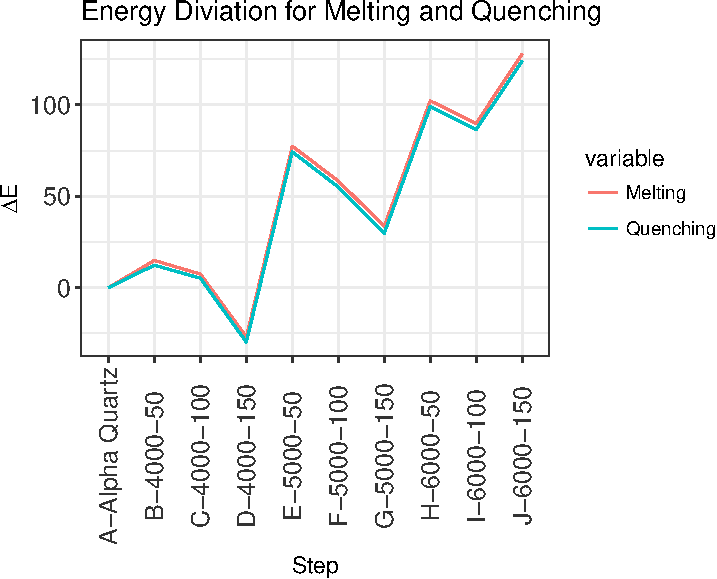
\includegraphics{merge_files/figure-latex/Graph: Energy diviation MQ-1.pdf}

Figure 1: Energy per experemental step

\hypertarget{section-1}{%
\subparagraph{.}\label{section-1}}

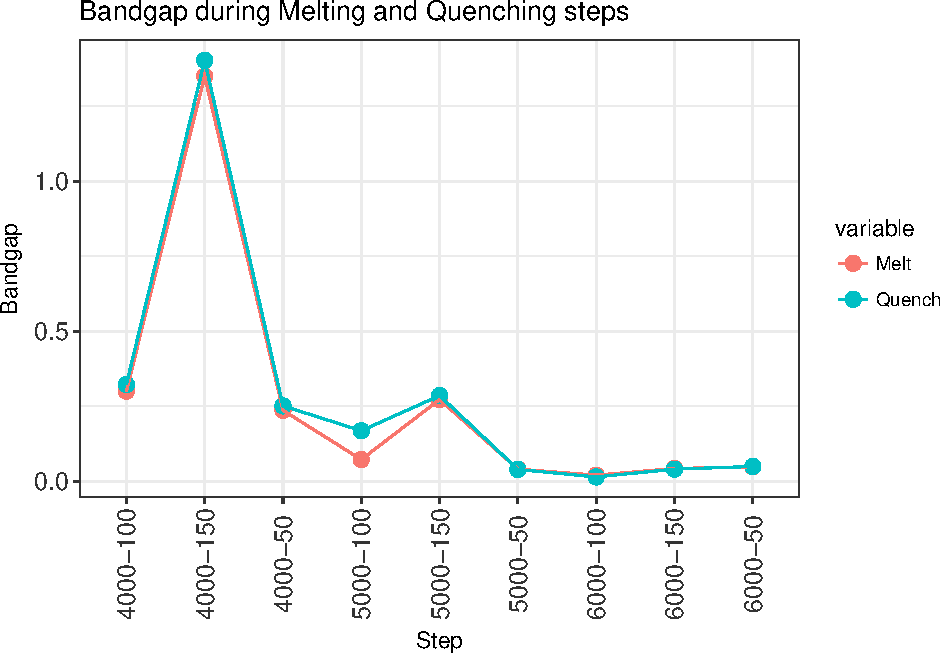
\includegraphics{merge_files/figure-latex/Graph: Bandgap Melt Quenching-1.pdf}

Figure 2: Bandgap during Melting and Quenching steps

As we expected (Figure 2) conclude that the band gap decreases as the
temperature and reaction time increase. Therefore as the alpha-quartz
become amorphous, there is also an increase in reactivity as seen in
(Figure 1).

\hypertarget{bond-angle-diviation}{%
\paragraph{Bond Angle diviation}\label{bond-angle-diviation}}

\begin{longtable}[]{@{}llrrrr@{}}
\toprule
& Step & \(\Delta\theta\) Melting & \(\Delta\theta\) Quenching &
\(\Delta\theta\) Annealing & \(\Delta\theta\) Cooling\tabularnewline
\midrule
\endhead
1 & 4000-50 & 6.324 & 6.271 & 0.737 & 5.433\tabularnewline
2 & 4000-100 & 19.665 & 19.577 & 1.865 & 10.574\tabularnewline
3 & 4000-150 & 12.045 & 11.999 & 1.940 & 15.151\tabularnewline
4 & 5000-50 & 19.225 & 19.246 & 10.141 & 2.409\tabularnewline
5 & 5000-100 & 19.180 & 19.144 & 6.154 & 4.549\tabularnewline
6 & 5000-150 & 30.070 & 30.001 & 9.275 & 30.070\tabularnewline
7 & 6000-50 & 26.742 & 26.646 & 6.604 & 26.646\tabularnewline
8 & 6000-100 & 35.009 & 34.938 & 23.254 & 18.168\tabularnewline
9 & 6000-150 & 11.029 & 10.946 & 15.867 & 15.867\tabularnewline
\bottomrule
\end{longtable}

Table 2: Bond angle diviation

\hypertarget{section-2}{%
\subparagraph{.}\label{section-2}}

\hypertarget{experimental-data}{%
\subsubsection{3. Experimental data}\label{experimental-data}}

\begin{longtable}[]{@{}llll@{}}
\toprule
& Info & \(\Delta \theta\) deg & \(\Delta\) E\tabularnewline
\midrule
\endhead
1 & Experimental & 10.8 & 0.28\tabularnewline
2 & Structural parameters of the unrelaxed amorphous silica & 17.7 &
0.19\tabularnewline
\bottomrule
\end{longtable}

Table 3: Literature results obtained at 4000K

\begin{center}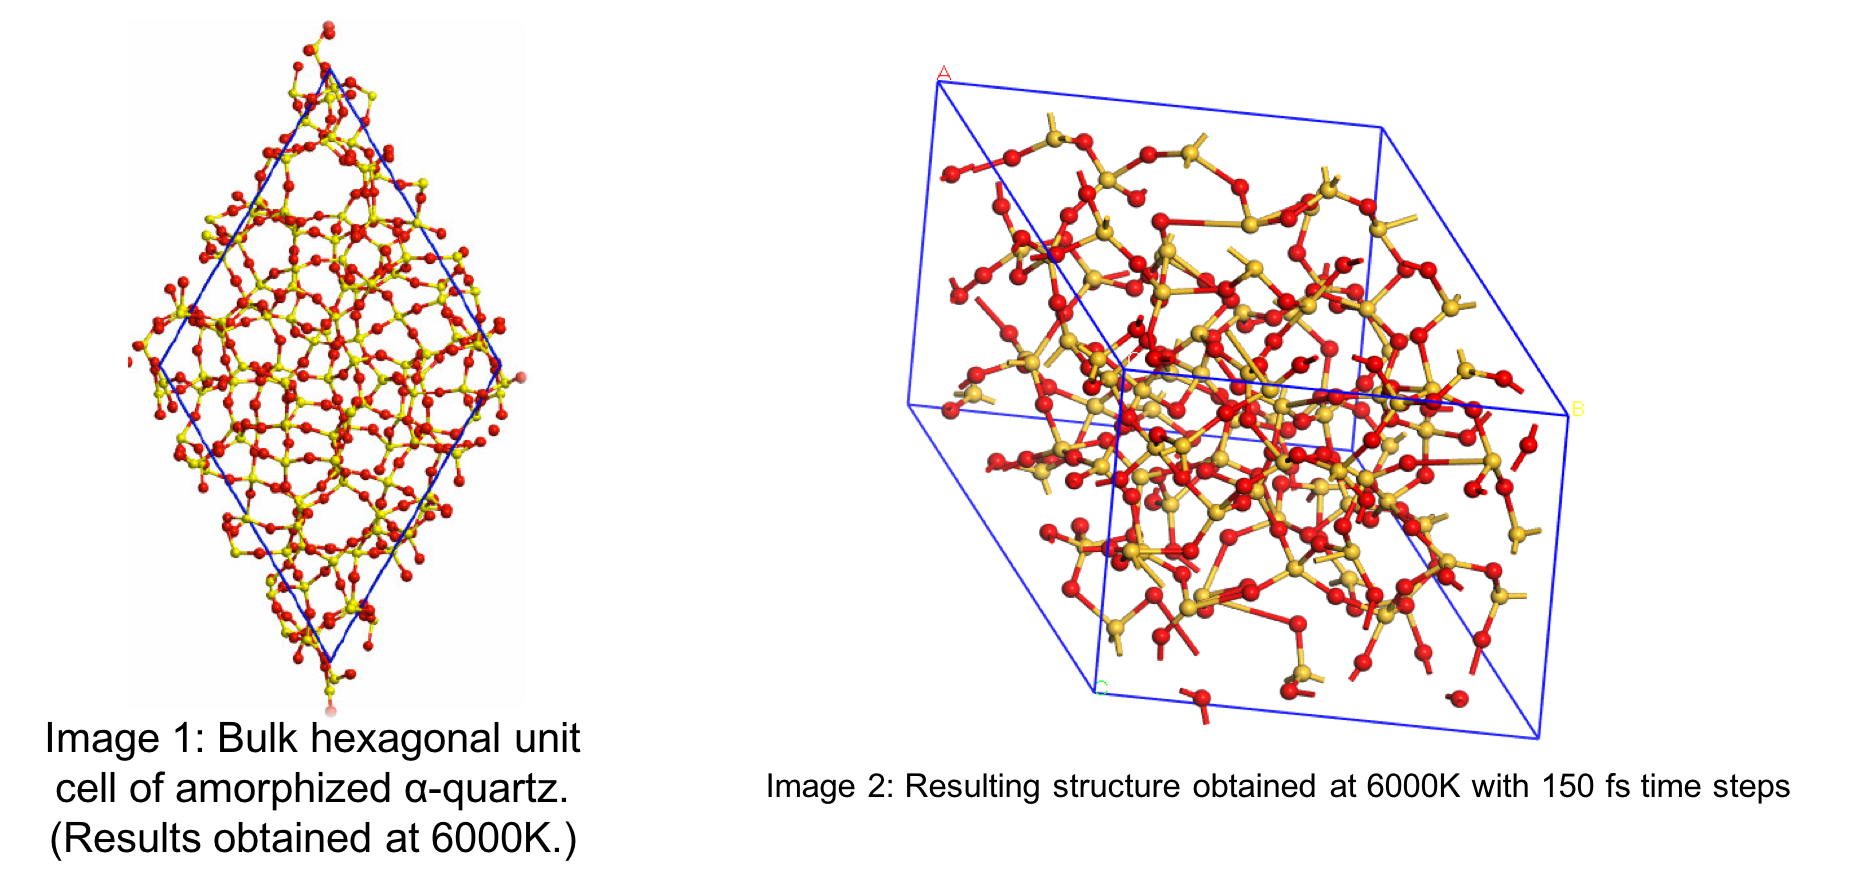
\includegraphics[width=0.9\linewidth]{../Report1/DATA/amorph-pics} \end{center}

Figure 3: Literature vs Experimental structional results(Izumi \emph{et
al.}, 2004)

\hypertarget{conclusion}{%
\subsubsection{4. Conclusion}\label{conclusion}}

\begin{itemize}
\tightlist
\item
  The bond angle deviation shown in (Table 2) can be related to
  experimental data obtained as seen in (Table 3).
\item
  At 4000K the \(\Delta\)Ε correlate with the experimental values
  obtained in (Table 3).
\end{itemize}

\hypertarget{section-3}{%
\subparagraph{.}\label{section-3}}

\hypertarget{modeling-sio2-surface}{%
\subsection{\texorpdfstring{2. Modeling SiO\textsubscript{2}
surface}{2. Modeling SiO2 surface}}\label{modeling-sio2-surface}}

To do surface calculations it became very difficult, using the amorphous
SiO2 bulk. We decide to use a crystalline 3X3X3 SiO2 bulk, using VASP
5.3. An Ab Initio Molecular Dynamics study will be done on all surfaces
using VASP 5.3.

\hypertarget{k-point-convergence-for-bulk-sio2-alpha-quartz}{%
\subsubsection{\texorpdfstring{K-point convergence for bulk
SiO\textsubscript{2} (Alpha
Quartz)}{K-point convergence for bulk SiO2 (Alpha Quartz)}}\label{k-point-convergence-for-bulk-sio2-alpha-quartz}}

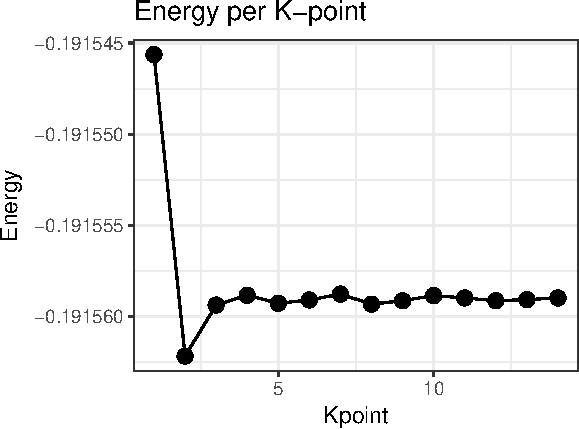
\includegraphics{merge_files/figure-latex/Graph:K-point convergence-1.pdf}

\hypertarget{sio2-surface-characterristics}{%
\subsubsection{\texorpdfstring{SiO\textsubscript{2} surface
characterristics}{SiO2 surface characterristics}}\label{sio2-surface-characterristics}}

The following surface characteristics will be determined

\begin{enumerate}
\def\labelenumi{\arabic{enumi}.}
\tightlist
\item
  Cutting planes: I will focus on the planes (100,110,200) as indicated
  in the XRD results see (Figure 5)
\end{enumerate}

\begin{center}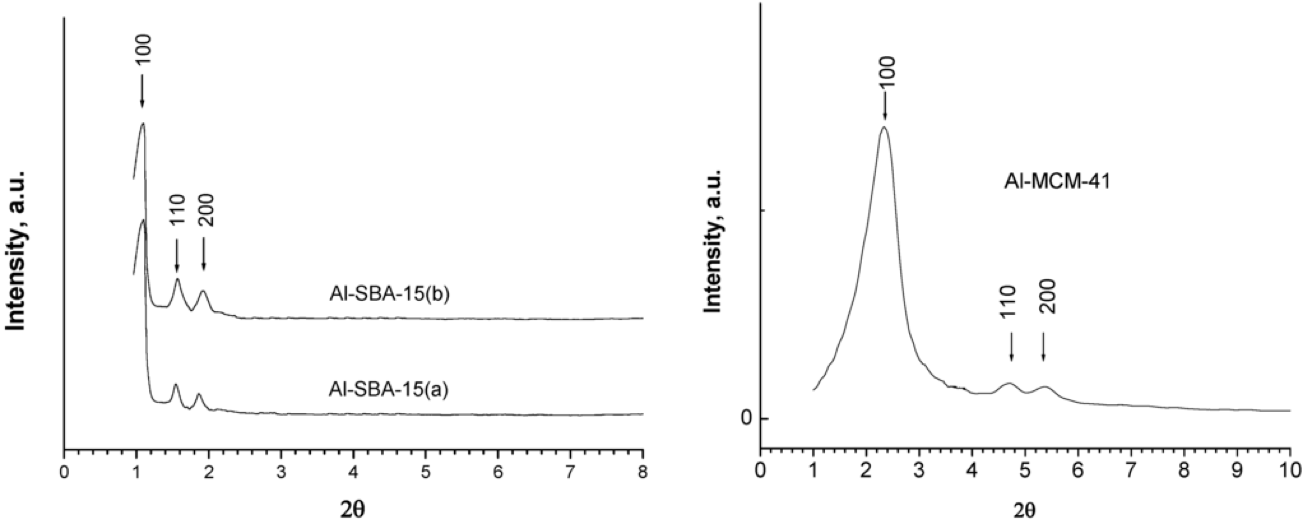
\includegraphics[width=0.9\linewidth]{../Report1/DATA/planes} \end{center}

Figure 5: XRD Data

\begin{itemize}
\item
  For each plane the following characteristics will be determined

  \begin{itemize}
  \item
    Slab Thickness
  \item
    Vacuum Gap size
  \item
    Surface thickness (The number of unrelaxed surface layers)
  \end{itemize}
\end{itemize}

\begin{enumerate}
\def\labelenumi{\arabic{enumi}.}
\setcounter{enumi}{1}
\item
  Create a amorphous surface layer from the ideal surface determined
  from characteristics obtained above.
\item
  Compare the amorphous surface reactivate with the crystalline surface
\end{enumerate}

\hypertarget{section-4}{%
\subparagraph{.}\label{section-4}}

\hypertarget{references}{%
\subsection{References}\label{references}}

\hypertarget{section-5}{%
\subparagraph{}\label{section-5}}

\hypertarget{section-6}{%
\subparagraph{}\label{section-6}}

\hypertarget{abstract}{%
\section{Abstract}\label{abstract}}

Three \(\alpha\)-Quartz ,spacegroup 180, surfaces were modelled using
crystallographic data from pearson\ldots{}. obtained in the Medea
package database. Surface planes with miller indexes 100, 110 and 200
were cut from the bulk structure. The different surfaces were compared
to identify the ideal MCM-41 surface to be used as a catalyst support.

\hypertarget{introduction-1}{%
\section{Introduction}\label{introduction-1}}

The utilisation of homogeneos catalysts in industry are limited, due to
the fact that it is expensive to extract the catalyst from post-reaction
mixtures (Balcar \& Čejka, 2013), (Kotzé, 2015). Research especialy in
the pharmaseutlical and petrochemistry industries took an intrest in the
imobilisation or heteroganasion of a homgeneous catalyst as a posible
solution to the mentiond problem.

Although the activity and selectivity of heterogeneous catalytic
reactions are lower than homogeneous reactions, the advantage of
separation, recovery and recycling outweigh these shortcomings. It is
however important to ensure that the effectiveness of the immobilized
homogeneous catalyst is not dramatically compromised (Kotzé, 2015),
(Gryp \emph{et al.}, 2010). Therefore the main objective in the
successful immobilization of homogeneous catalyst systems is to combine
the high activity and selectivity properties of homogeneous catalysts
with the ease of recovery of a heterogeneous catalyst. To accomplish
this the selection of an appropriate support material is very important
(Kotzé, 2015).

Support materials can be divided into three categories e.g.~insoluble
organic, polymeric or inorganic supports. Immobilization by using
insoluble organic supports involves ultrafiltration techniques as seen
in the separation of the PUK-Grubbs 2 catalyst by using organic solvent
nanofiltration (Gryp \emph{et al.}, 2010). Van der Gryp et al. (Gryp
\emph{et al.}, 2010) performed this separation using organic membranes
and discovered that the catalyst can be successfully separated, but its
lifetime was dramatically decreased during the filtration process (Gryp
\emph{et al.}, 2010), (Kotzé, 2015). Polymer supports on the other hand
provide easier filtration techniques, multiple coordination sites and
the possibility to incorporate a molecular catalyst into the polymer
structure. These are great advantages, but during the filtration process
the thermal stability remains low (Kotzé, 2015). Inorganic supports have
a high thermal stability, it provides for multiple coordination sites
because it contains a large surface area (BET), big pores and narrow
pore size distributions. Therefore inorganic supports are more effective
in the immobilization of homogeneous catalysts systems than organic or
polymeric support surfaces.(Balcar \& Čejka, 2013)

There are three types of inorganic supports available, which is
categorized by their pore sizes and physical compositions:

\begin{enumerate}
\def\labelenumi{\arabic{enumi}.}
\tightlist
\item
  Inorganic microporous support materials have pore sizes \textless{}
  2nm, e.g.~Zeolites, Metal-Organic Frameworks (MOFs);
\item
  Inorganic mesoporous support materials have pore sizes in the range of
  2-15 nm, e.g.~MCM-41, SBA-15 and Aerogels; and
\item
  Inorganic macroporous support materials have pore sizes greater than
  50 nm, e.g.~glasses. (Balcar \& Čejka, 2013), (Kotzé, 2015)
\end{enumerate}

Although microporous and macroporious support materials have the ability
to be used as heterogeneous support, it doesn't have an industrial
appeal yet (Balcar \& Čejka, 2013),(Kotzé, 2015). Therefore the focus is
on mesoporous support materials. Since the successful synthesis of
mesoporous materials by Mobil in 1992, the research field in using and
synthesizing mesoporious materials as support materials for
heterogeneous catalytic reactions has grown significantly. The original
synthesis of mesoporous support material was defined as the M41S family
containing hexagonal MCM-41, cubic MCM-48 and lamellar MCM-50
structures. A more visual representation of the different structures can
be seen in Figure 6

\begin{center}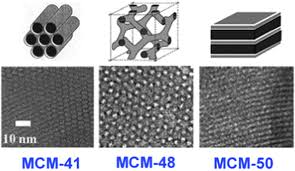
\includegraphics[width=0.9\linewidth]{Data/Images/Mcm-structures} \end{center}

Figure 6: Different structures of the M41S family (Linares \emph{et
al.}, 2014)

Unfortunately M41S materials have a limitation in pore diameter,
approximately 80 Å, which affects the separation of large molecules
(Katiyar \emph{et al.}, 2006). Zhao et al. (Zhao \emph{et al.}, 1998)
extended the family of inorganic mesoporous support materials by
synthesizing Santa Barbara Amorphous (SBA) type materials, with a pore
diameter ranging between 20 to 300 Å.

\hypertarget{surface-characterization}{%
\subsection{Surface characterization}\label{surface-characterization}}

The surface of mesoporous support materials are amporphious and contain
accessible hydroxyl groups. This makes immobilization of homogeneous
complexes on the silica surface possible (Kotzé, 2015). The crusial
factor for immobilization of a catalyst on the silica surface is the
concentration, distribution and accessibility of the silanol groups on
the silica surface (Balcar \& Čejka, 2013). Ramírez et al. (A. Ramı'rez
\& Sierra*, 2003) showed that the types of silanols present on the
silica surface are single, hydrogen bonded or germinal silanol groups as
shown in Figure 7.

\begin{center}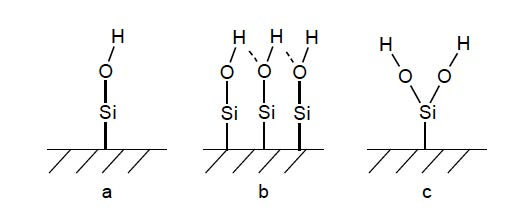
\includegraphics[width=7.11in]{Data/Images/Silanol_groups} \end{center}

Figure 7: Different silanol groups on the surface of a silica support:
(a) single, (b) hydrogen bonded and (c) geminal silanol groups {[}A.
Ramı'rez \& Sierra* (2003){]}

Coordination of the metal complexes to the support can either take place
by binding of the metal ions directly or via organic molecule linkers to
the silanols. Sels and co-workers (Van Berlo \emph{et al.}, 2008)
observed that a weak physical interaction between a neutral
Hoveyda-Grubbs- II type complex and the inorganic support was enough to
seperate the complex from the mixture and altered surfaces using linkers
was not nessesary. Cabrera et al. (Cabrera \emph{et al.}, 2012) and
Schachner et al. (Schachner \emph{et al.}, 2011) also found that
ruthenium-based metathesis catalysts containing a hemilabile
pyridine-alkoxide ligand adsorb extremely well onto an unmodified silica
support without compromising too much on the homogeneous catalytic
effectiveness.

\hypertarget{experimental}{%
\section{Experimental}\label{experimental}}

\hypertarget{results-and-discussion}{%
\section{Results and discussion}\label{results-and-discussion}}

\listoffigures

\hypertarget{refs}{}
\leavevmode\hypertarget{ref-RN75}{}%
A. Ramı'rez, B. L. Lopez \& Sierra*, L. 2003. Study of the acidic sites
and their modifications in mesoporous silica synthesized in acidic
medium under quiescent conditions. \emph{Journal of Physical Chemistry}.
(107):5.

\leavevmode\hypertarget{ref-RN44}{}%
Balcar, H. \& Čejka, J. 2013. Mesoporous molecular sieves as advanced
supports for olefin metathesis catalysts. \emph{Coordination Chemistry
Reviews}. 257(21-22):3107--3124.

\leavevmode\hypertarget{ref-RN84}{}%
Cabrera, J., Padilla, R., Bru, M., Lindner, R., Kageyama, T., Wilckens,
K., Balof, S.L., Schanz, H.J., Dehn, R., Teles, J.H., Deuerlein, S.,
Muller, K., Rominger, F., \& Limbach, M. 2012. Linker-free, silica-bound
olefin-metathesis catalysts: Applications in heterogeneous catalysis.
\emph{Chemistry}. 18(46):14717--24.

\leavevmode\hypertarget{ref-Rep1}{}%
Group, T.S. 2014. Overview of silica polymorphs.

\leavevmode\hypertarget{ref-RN73}{}%
Gryp, P. van der, Barnard, A., Cronje, J.-P., Vlieger, D. de, Marx, S.,
\& Vosloo, H.C.M. 2010. Separation of different metathesis grubbs-type
catalysts using organic solvent nanofiltration. \emph{Journal of
Membrane Science}. 353(1-2):70--77.

\leavevmode\hypertarget{ref-RN96}{}%
Izumi, S., Hara, S., Kumagai, T., \& Sakai, S. 2004. Classification of
amorphous-silicon microstructures by structural parameters: Molecular
dynamics study. \emph{Computational Materials Science}.
31(3-4):258--268.

\leavevmode\hypertarget{ref-RN88}{}%
Jordaan, M. 2007. Experimental and theoretical investigation of new
grubbs-mae catalysts for the metathesis of alkenes (Journal Article).
North West University South Africa.

\leavevmode\hypertarget{ref-RN89}{}%
Katiyar, A., Yadav, S., Smirniotis, P.G., \& Pinto, N.G. 2006. Synthesis
of ordered large pore sba-15 spherical particles for adsorption of
biomolecules. \emph{J Chromatogr A}. 1122(1-2):13--20.

\leavevmode\hypertarget{ref-RN90}{}%
Kotzé, H. de V. 2015. Immobilized ru(II) catalysts for transfer
hydrogenation and oxidative alkene cleavage reactions (Journal Article).
Stellenbosh University South Africa.

\leavevmode\hypertarget{ref-RN87}{}%
Linares, N., Silvestre-Albero, A.M., Serrano, E., Silvestre-Albero, J.,
\& Garcia-Martinez, J. 2014. Mesoporous materials for clean energy
technologies. \emph{Chem Soc Rev}. 43(22):7681--717.

\leavevmode\hypertarget{ref-RN85}{}%
Schachner, J.A., Cabrera, J., Padilla, R., Fischer, C., Schaaf, P.A. van
der, Pretot, R., Rominger, F., \& Limbach, M. 2011. A set of olefin
metathesis catalysts with extraordinary stickiness to silica. \emph{ACS
Catalysis}. 1(8):872--876.

\leavevmode\hypertarget{ref-RN92}{}%
Thielemann, J.P., Girgsdies, F., Schlogl, R., \& Hess, C. 2011. Pore
structure and surface area of silica sba-15: Influence of washing and
scale-up. \emph{Beilstein J Nanotechnol}. 2:110--8.

\leavevmode\hypertarget{ref-RN13}{}%
Ugliengo, P., Sodupe, M., Musso, F., Bush, I.J., Orlando, R., \& Dovesi,
R. 2008. Realistic models of hydroxylated amorphous silica surfaces and
mcm-41 mesoporous material simulated by large-scale periodic b3lyp
calculations. \emph{Advanced Materials}. 20(23):4579--4583.

\leavevmode\hypertarget{ref-RN74}{}%
Van Berlo, B., Houthoofd, K., Sels, B., \& Jacobs, P. 2008. Silica
immobilized second generation hoveyda-grubbs: A convenient, recyclable
and storageable heterogeneous solid catalyst. \emph{Advanced Synthesis
\& Catalysis}. 350(13):1949--1953.

\leavevmode\hypertarget{ref-RN69}{}%
Zhao, D., Feng, J., Huo, Q., Melosh, N., Fredrickson, G.H., Chmelka,
B.F., \& Stucky, G.D. 1998. Triblock copolymer syntheses of mesoporous
silica with periodic 50 to 300 angstrom pores. \emph{SCIENCE}. 279(548).


\end{document}
